% ====================================================================
% ФАЙЛ: tasks/03_electrodynamics/circuits_and_ohms_law_full_part1.tex
% ТЕМА: СОЕДИНЕНИЕ ПРОВОДНИКОВ. ЗАКОН ОМА ДЛЯ ПОЛНОЙ ЦЕПИ
% ПАЧКА 1: ВАРИАНТЫ 1–10
% ====================================================================

% === ЗАДАЧА 1 ===
% Тег: #ЭЛЕКТРОДИНАМИКА #ТОК #ЗАКОН_ОМА_ПОЛНАЯ_ЦЕПЬ #КИМ_11 #ВАРИАНТ_01
\begin{taskbasic}[code={\label{task:elem_circ_v1_n11}}]
\textbf{Задача 1.} Источник тока с электродвижущей силой $\mathcal{E} = 6\text{ В}$ и внутренним сопротивлением $r = 1\text{ Ом}$ замкнут на резистор сопротивлением $R = 2\text{ Ом}$. Чему равна сила тока в цепи? Ответ выразите в амперах (А).

\kim{11}
\end{taskbasic}
\answer{2}

% === ЗАДАЧА 2 ===
% Тег: #ЭЛЕКТРОДИНАМИКА #ТОК #СОЕДИНЕНИЕ_ПРОВОДНИКОВ #КИМ_11 #ВАРИАНТ_02
\begin{taskbasic}[code={\label{task:elem_circ_v2_n11}}]
\textbf{Задача 2.} Чему равно общее электрическое сопротивление участка цепи, состоящего из двух параллельно соединённых резисторов сопротивлением $R_1 = 20\text{ Ом}$ и $R_2 = 30\text{ Ом}$? Ответ выразите в омах (Ом).

\nopagebreak\smallskip
\begin{center}
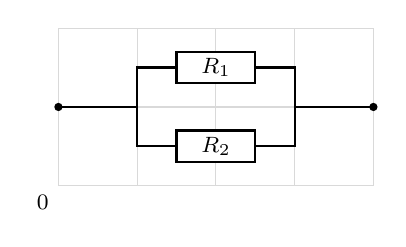
\begin{tikzpicture}[scale=1.0, every node/.style={font=\footnotesize}]
    \draw[xstep=1, ystep=1, gray!30, thin] (0,0) grid (4,2);
    
    % Вход и выход
    \draw[thick, black] (0,1) -- (1,1);
    \draw[thick, black] (3,1) -- (4,1);
    
    % Разветвление
    \draw[thick, black] (1,1) -- (1,0.5) -- (1.5,0.5);
    \draw[thick, black] (1,1) -- (1,1.5) -- (1.5,1.5);
    \draw[thick, black] (2.5,0.5) -- (3,0.5) -- (3,1);
    \draw[thick, black] (2.5,1.5) -- (3,1.5) -- (3,1);
    
    % Резисторы
    \draw[thick, black, fill=white] (1.5,1.3) rectangle (2.5,1.7) node[pos=.5] {$R_1$};
    \draw[thick, black, fill=white] (1.5,0.3) rectangle (2.5,0.7) node[pos=.5] {$R_2$};
    
    % Клеммы
    \fill[black] (0,1) circle (1.5pt);
    \fill[black] (4,1) circle (1.5pt);
    
    \node[below left] at (0,0) {0};
\end{tikzpicture}
\end{center}

\kim{11}
\end{taskbasic}
\answer{12}

% === ЗАДАЧА 3 ===
% Тег: #ЭЛЕКТРОДИНАМИКА #ТОК #ЗАКОН_ОМА_ПОЛНАЯ_ЦЕПЬ #КИМ_14 #ВАРИАНТ_05
\begin{taskbasic}[code={\label{task:elem_circ_v5_n14}}]
\textbf{Задача 3.} Источник тока с ЭДС $\mathcal{E}$ и внутренним сопротивлением $r$ замкнут на реостат. При изменении сопротивления реостата измерялись сила тока $I$ в цепи и напряжение $U$ на зажимах источника. Из приведённого ниже списка выберите все верные утверждения относительно процессов в этой цепи.

\nopagebreak\smallskip
\begin{center}
\begin{tikzpicture}[scale=1.0, every node/.style={font=\footnotesize}]
    \draw[xstep=1, ystep=1, gray!30, thin] (0,0) grid (4,3);
    
    % Оси координат
    \draw[-{Stealth[scale=0.8]}, black, thick] (0,0) -- (4.5,0) node[right] {$I$, А};
    \draw[-{Stealth[scale=0.8]}, black, thick] (0,0) -- (0,3.5) node[above] {$U$, В};
    
    % График U(I) = E - Ir
    \draw[ultra thick, brandPrimary] (0,2.5) -- (3.5,0.5);
    
    \fill[black] (0,2.5) circle (1.5pt) node[left] {$\mathcal{E}$};
    \fill[black] (3.5,0.5) circle (1.5pt);
    
    \draw[dashed, gray] (3.5,0) -- (3.5,0.5);
    \draw[dashed, gray] (0,0.5) -- (3.5,0.5);
    
    \node[left] at (0,0.5) {$U_1$};
    \node[below] at (3.5,0) {$I_1$};
    \node[below left] at (0,0) {0};
\end{tikzpicture}
\end{center}

1) При уменьшении сопротивления реостата напряжение на зажимах источника уменьшается.\\
2) Ток короткого замыкания источника равен $I_1$.\\
3) Электродвижущая сила источника равна $U_1$.\\
4) Внутреннее сопротивление источника можно определить по наклону графика $U(I)$.\\
5) При увеличении сопротивления реостата сила тока в цепи увеличивается.

\kim{14}
\end{taskbasic}
\answer{14}

% === ЗАДАЧА 4 ===
% Тег: #ЭЛЕКТРОДИНАМИКА #ТОК #ЗАКОН_ОМА_ПОЛНАЯ_ЦЕПЬ #КИМ_25 #ВАРИАНТ_06
\begin{taskbasic}[code={\label{task:elem_circ_v6_n25}}]
\textbf{Задача 4.} К источнику тока с ЭДС $\mathcal{E} = 12\text{ В}$ подключены три одинаковых резистора сопротивлением $R = 5\text{ Ом}$ каждый, соединённых последовательно. При этом сила тока в цепи равна $I = 0{,}75\text{ А}$. Определите внутреннее сопротивление $r$ источника тока. Ответ выразите в омах (Ом).

\kim{25}
\end{taskbasic}
\answer{1}

% ====================================================================
% ФАЙЛ: tasks/03_electrodynamics/circuits_and_ohms_law_full_part2.tex
% ТЕМА: СОЕДИНЕНИЕ ПРОВОДНИКОВ. ЗАКОН ОМА ДЛЯ ПОЛНОЙ ЦЕПИ
% ПАЧКА 2: ВАРИАНТЫ 11–20
% ====================================================================

% === ЗАДАЧА 1 ===
% Тег: #ЭЛЕКТРОДИНАМИКА #ТОК #СОЕДИНЕНИЕ_ПРОВОДНИКОВ #КИМ_11 #ВАРИАНТ_11
\begin{taskbasic}[code={\label{task:elem_circ_v11_n11}}]
\textbf{Задача 1.} Во сколько раз уменьшится общее сопротивление участка цепи, состоящего из двух одинаковых резисторов, если их последовательное соединение заменить на параллельное?

\kim{11}
\end{taskbasic}
\answer{3}

% === ЗАДАЧА 2 ===
% Тег: #ЭЛЕКТРОДИНАМИКА #ТОК #СОЕДИНЕНИЕ_ПРОВОДНИКОВ #КИМ_11 #ВАРИАНТ_12
\begin{taskbasic}[code={\label{task:elem_circ_v12_n11}}]
\textbf{Задача 2.} Чему равно общее электрическое сопротивление участка цепи, состоящего из двух последовательно соединённых резисторов сопротивлением $R_1 = 10\text{ Ом}$ и $R_2 = 14\text{ Ом}$? Ответ выразите в омах (Ом).

\nopagebreak\smallskip
\begin{center}
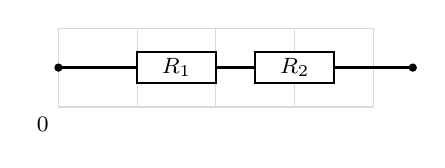
\begin{tikzpicture}[scale=1.0, every node/.style={font=\footnotesize}]
    \draw[xstep=1, ystep=1, gray!30, thin] (0,0) grid (4,1);
    
    \draw[thick, black] (0,0.5) -- (1,0.5);
    \draw[thick, black, fill=white] (1,0.3) rectangle (2,0.7) node[pos=.5] {$R_1$};
    \draw[thick, black] (2,0.5) -- (2.5,0.5);
    \draw[thick, black, fill=white] (2.5,0.3) rectangle (3.5,0.7) node[pos=.5] {$R_2$};
    \draw[thick, black] (3.5,0.5) -- (4.5,0.5);
    
    \fill[black] (0,0.5) circle (1.5pt);
    \fill[black] (4.5,0.5) circle (1.5pt);
    
    \node[below left] at (0,0) {0};
\end{tikzpicture}
\end{center}

\kim{11}
\end{taskbasic}
\answer{24}

% === ЗАДАЧА 3 ===
% Тег: #ЭЛЕКТРОДИНАМИКА #ТОК #ЗАКОН_ОМА_ПОЛНАЯ_ЦЕПЬ #КИМ_14 #ВАРИАНТ_15
\begin{taskbasic}[code={\label{task:elem_circ_v15_n14}}]
\textbf{Задача 3.} Электрическая цепь состоит из источника тока с ЭДС $\mathcal{E}$ и внутренним сопротивлением $r$, резистора $R$ и реостата, соединённых последовательно. Ползунок реостата перемещают так, что его сопротивление уменьшается. Из приведённого ниже списка выберите все верные утверждения относительно произошедших изменений.

\nopagebreak\smallskip
\begin{center}
\begin{tikzpicture}[scale=1.0, every node/.style={font=\footnotesize}]
    \draw[xstep=1, ystep=1, gray!30, thin] (0,0) grid (4,3);
    
    % Схема цепи
    \draw[thick, black] (0.5,0.5) rectangle (3.5,2.5);
    
    % Источник
    \fill[white] (0.5,1.1) rectangle (0.5,1.9);
    \draw[thick, black] (0.5,1.1) -- (0.5,1.4);
    \draw[thick, black] (0.2,1.4) -- (0.8,1.4);
    \draw[ultra thick, black] (0.35,1.6) -- (0.65,1.6);
    \draw[thick, black] (0.5,1.6) -- (0.5,1.9);
    
    % Резистор
    \draw[thick, black, fill=white] (1.5,2.3) rectangle (2.5,2.7) node[pos=.5] {$R$};
    
    % Реостат
    \draw[thick, black, fill=white] (1.5,0.3) rectangle (2.5,0.7);
    \draw[-{Stealth[scale=0.8]}, thick, black] (2.0,1.1) -- (2.0,0.7);
    
    \node[below left] at (0,0) {0};
\end{tikzpicture}
\end{center}

1) Сила тока в цепи увеличивается.\\
2) Напряжение на зажимах источника тока увеличивается.\\
3) Обще сопротивление цепи увеличивается.\\
4) Напряжение на резисторе $R$ увеличивается.\\
5) Мощность, выделяемая на внутреннем сопротивлении источника, уменьшается.

\kim{14}
\end{taskbasic}
\answer{14}

% === ЗАДАЧА 4 ===
% Тег: #ЭЛЕКТРОДИНАМИКА #ТОК #ЗАКОН_ОМА_ПОЛНАЯ_ЦЕПЬ #КИМ_25 #ВАРИАНТ_16
\begin{taskbasic}[code={\label{task:elem_circ_v16_n25}}]
\textbf{Задача 4.} Источник тока с ЭДС $\mathcal{E} = 6\text{ В}$ и внутренним сопротивлением $r$ питает цепь, состоящую из двух параллельно соединённых резисторов сопротивлением $R_1 = 4\text{ Ом}$ и $R_2 = 12\text{ Ом}$. Сила тока в неразветвлённой части цепи равна $I = 1{,}5\text{ А}$. Чему равно внутреннее сопротивление $r$ источника тока? Ответ выразите в омах (Ом).

\kim{25}
\end{taskbasic}
\answer{0,5}

% ====================================================================
% ФАЙЛ: tasks/03_electrodynamics/circuits_and_ohms_law_full_part3.tex
% ТЕМА: СОЕДИНЕНИЕ ПРОВОДНИКОВ. ЗАКОН ОМА ДЛЯ ПОЛНОЙ ЦЕПИ
% ПАЧКА 3: ВАРИАНТЫ 21–30
% ====================================================================

% === ЗАДАЧА 1 ===
% Тег: #ЭЛЕКТРОДИНАМИКА #ТОК #СОЕДИНЕНИЕ_ПРОВОДНИКОВ #КИМ_11 #ВАРИАНТ_21
\begin{taskbasic}[code={\label{task:elem_circ_v21_n11}}]
\textbf{Задача 1.} Чему равно общее электрическое сопротивление участка цепи, состоящего из двух последовательно соединённых резисторов сопротивлением $R_1 = 6\text{ Ом}$ и $R_2 = 9\text{ Ом}$? Ответ выразите в омах (Ом).

\kim{11}
\end{taskbasic}
\answer{15}

% === ЗАДАЧА 2 ===
% Тег: #ЭЛЕКТРОДИНАМИКА #ТОК #ЗАКОН_ОМА_ПОЛНАЯ_ЦЕПЬ #КИМ_11 #ВАРИАНТ_22
\begin{taskbasic}[code={\label{task:elem_circ_v22_n11}}]
\textbf{Задача 2.} Источник тока с ЭДС $\mathcal{E} = 9\text{ В}$ и внутренним сопротивлением $r = 1\text{ Ом}$ замкнут на два параллельно соединённых резистора сопротивлением $R_1 = 10\text{ Ом}$ и $R_2 = 10\text{ Ом}$. Чему равна сила тока в неразветвлённой части цепи? Ответ выразите в амперах (А).

\nopagebreak\smallskip
\begin{center}
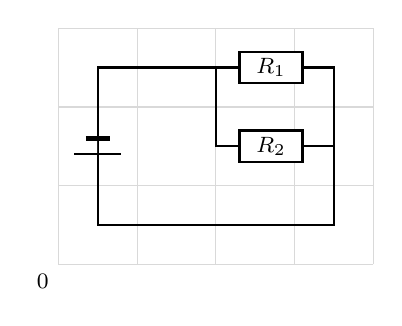
\begin{tikzpicture}[scale=1.0, every node/.style={font=\footnotesize}]
    \draw[xstep=1, ystep=1, gray!30, thin] (0,0) grid (4,3);
    
    % Внешняя контурная рамка цепи
    \draw[thick, black] (0.5,0.5) -- (0.5,2.5) -- (3.5,2.5) -- (3.5,0.5) -- cycle;
    
    % Источник тока (слева)
    \fill[white] (0.5,1.1) rectangle (0.5,1.9);
    \draw[thick, black] (0.5,1.1) -- (0.5,1.4);
    \draw[thick, black] (0.2,1.4) -- (0.8,1.4);
    \draw[ultra thick, black] (0.35,1.6) -- (0.65,1.6);
    \draw[thick, black] (0.5,1.6) -- (0.5,1.9);
    
    % Разветвление справа
    \draw[thick, black] (2.0,2.5) -- (2.0,1.5) -- (3.5,1.5);
    
    % Резистор R1
    \draw[thick, black, fill=white] (2.3,2.3) rectangle (3.1,2.7) node[pos=.5] {$R_1$};
    
    % Резистор R2
    \draw[thick, black, fill=white] (2.3,1.3) rectangle (3.1,1.7) node[pos=.5] {$R_2$};
    
    \node[below left] at (0,0) {0};
\end{tikzpicture}
\end{center}

\kim{11}
\end{taskbasic}
\answer{1,5}

% === ЗАДАЧА 3 ===
% Тег: #ЭЛЕКТРОДИНАМИКА #ТОК #ЗАКОН_ОМА_ПОЛНАЯ_ЦЕПЬ #КИМ_14 #ВАРИАНТ_25
\begin{taskbasic}[code={\label{task:elem_circ_v25_n14}}]
\textbf{Задача 3.} В электрической цепи, схема которой приведена на рисунке, идеальный вольтметр измеряет напряжение на зажимах источника тока. Сопротивление реостата плавно увеличивают. Из приведённого ниже списка выберите все верные утверждения относительно изменений показаний приборов.

\nopagebreak\smallskip
\begin{center}
\begin{tikzpicture}[scale=1.0, every node/.style={font=\footnotesize}]
    \draw[xstep=1, ystep=1, gray!30, thin] (0,0) grid (4,3);
    
    % Контур цепи
    \draw[thick, black] (0.5,0.5) rectangle (3.5,2.5);
    
    % Источник
    \fill[white] (0.5,1.1) rectangle (0.5,1.9);
    \draw[thick, black] (0.2,1.4) -- (0.8,1.4);
    \draw[ultra thick, black] (0.35,1.6) -- (0.65,1.6);
    
    % Амперметр
    \fill[white] (2.0,2.5) circle (0.3);
    \draw[thick, black] (2.0,2.5) circle (0.3) node {A};
    
    % Реостат
    \draw[thick, black, fill=white] (1.5,0.3) rectangle (2.5,0.7);
    \draw[-{Stealth[scale=0.8]}, thick, black] (2.0,1.1) -- (2.0,0.7);
    
    % Вольтметр (параллельно источнику)
    \draw[thick, black] (0.5,2.1) -- (1.0,2.1) -- (1.0,0.9) -- (0.5,0.9);
    \fill[white] (1.0,1.5) circle (0.3);
    \draw[thick, black] (1.0,1.5) circle (0.3) node {V};
    
    \node[below left] at (0,0) {0};
\end{tikzpicture}
\end{center}

1) Показания амперметра увеличиваются.\\
2) Показания вольтметра увеличиваются.\\
3) Общее сопротивление цепи уменьшается.\\
4) Сила тока короткого замыкания увеличивается.\\
5) Напряжение на зажимах источника приближается к его ЭДС.

\kim{14}
\end{taskbasic}
\answer{25}

% === ЗАДАЧА 4 ===
% Тег: #ЭЛЕКТРОДИНАМИКА #ТОК #ЗАКОН_ОМА_ПОЛНАЯ_ЦЕПЬ #КИМ_25 #ВАРИАНТ_26
\begin{taskbasic}[code={\label{task:elem_circ_v26_n25}}]
\textbf{Задача 4.} Источник тока с ЭДС $\mathcal{E} = 10\text{ В}$ и внутренним сопротивлением $r$ питает цепь, состоящую из двух параллельно соединённых резисторов $R_1 = 6\text{ Ом}$ и $R_2 = 12\text{ Ом}$. Напряжение на зажимах источника равно $U = 8\text{ В}$. Определите внутреннее сопротивление $r$ источника тока. Ответ выразите в омах (Ом).

\kim{25}
\end{taskbasic}
\answer{2}

% === ЗАДАЧА ===
% Тег: #ЭЛЕКТРОДИНАМИКА #ТОК #ДИОДЫ #КИМ_21
\begin{taskbasic}[code={\label{task:elem_circuit_diodes_k1_k2}}]
Электрическая цепь состоит из источника ЭДС, двух резисторов сопротивлениями $R_1$ и $R_2$, двух идеальных диодов (сопротивление диода при прямом включении равно нулю, при обратном включении ток через диод равен нулю), двух ключей и идеальных амперметра и вольтметра (см. рисунок). В начальный момент времени ключ $K_1$ разомкнут, а ключ $K_2$ замкнут. Опираясь на законы электродинамики, объясните, как изменятся показания приборов, если ключ $K_1$ замкнуть, а ключ $K_2$ разомкнуть.

\nopagebreak\smallskip
\begin{center}
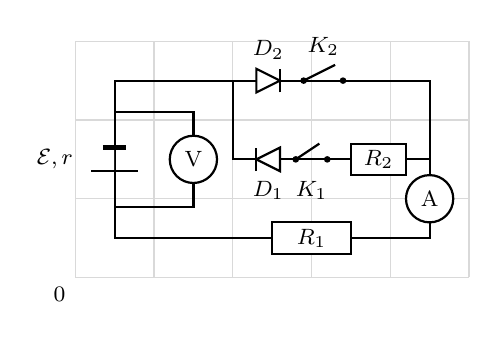
\begin{tikzpicture}[scale=1.0, every node/.style={font=\footnotesize}]
    \draw[xstep=1, ystep=1, gray!30, thin] (0,0) grid (5,3);
    
    % Внешний контур
    \draw[thick, black] (0.5,0.5) -- (0.5,2.5) -- (4.5,2.5) -- (4.5,0.5) -- cycle;
    
    % Источник тока (слева)
    \fill[white] (0.5,1.0) rectangle (0.5,2.0);
    \draw[thick, black] (0.5,1.0) -- (0.5,1.35);
    \draw[thick, black] (0.2,1.35) -- (0.8,1.35);
    \draw[ultra thick, black] (0.35,1.65) -- (0.65,1.65);
    \draw[thick, black] (0.5,1.65) -- (0.5,2.0);
    \node[left=3pt] at (0.2,1.5) {$\mathcal{E}, r$};
    
    % Вольтметр (параллельно источнику)
    \draw[thick, black] (0.5,2.1) -- (1.5,2.1) -- (1.5,0.9) -- (0.5,0.9);
    \fill[white] (1.5,1.5) circle (0.3);
    \draw[thick, black] (1.5,1.5) circle (0.3) node {V};
    
    % Разветвление на 2 диода
    \draw[thick, black] (2.0,2.5) -- (2.0,1.5) -- (4.5,1.5);
    
    % Верхняя ветвь (D2, K2)
    \draw[thick, black, fill=white] (2.3,2.35) -- (2.3,2.65) -- (2.6,2.5) -- cycle;
    \draw[thick, black] (2.6,2.35) -- (2.6,2.65);
    \node[above] at (2.45,2.65) {$D_2$};
    \fill[black] (2.9,2.5) circle (1.2pt);
    \fill[black] (3.4,2.5) circle (1.2pt);
    \draw[thick, black] (2.9,2.5) -- (3.3,2.7);
    \node[above] at (3.15,2.7) {$K_2$};
    
    % Нижняя ветвь (D1, K1, R2)
    \draw[thick, black, fill=white] (2.6,1.35) -- (2.6,1.65) -- (2.3,1.5) -- cycle;
    \draw[thick, black] (2.3,1.35) -- (2.3,1.65);
    \node[below] at (2.45,1.35) {$D_1$};
    \fill[black] (2.8,1.5) circle (1.2pt);
    \fill[black] (3.2,1.5) circle (1.2pt);
    \draw[thick, black] (2.8,1.5) -- (3.1,1.7);
    \node[below] at (3.0,1.35) {$K_1$};
    \draw[thick, black, fill=white] (3.5,1.3) rectangle (4.2,1.7) node[pos=.5] {$R_2$};
    
    % Амперметр (справа)
    \fill[white] (4.5,1.0) circle (0.3);
    \draw[thick, black] (4.5,1.0) circle (0.3) node {A};
    
    % Резистор R1 (снизу)
    \draw[thick, black, fill=white] (2.5,0.3) rectangle (3.5,0.7) node[pos=.5] {$R_1$};
    
    \node[below left] at (0,0) {0};
\end{tikzpicture}
\end{center}

\kim{21}
\end{taskbasic}
\answer{Показания амперметра уменьшатся до нуля, показания вольтметра увеличатся}